\documentclass[times, twoside, watermark]{zHenriquesLab-StyleBioRxiv}
\usepackage{blindtext}

% Please give the surname of the lead author for the running footer
\leadauthor{Koen Rademaker} 

\begin{document}

\title{Innovations in multimodal single-cell sequencing}

\shorttitle{Literature Review}

% Use letters for affiliations, numbers to show equal authorship (if applicable) and to indicate the corresponding author
\author[1]{Koen Rademaker}
\affil[1]{MSc student Bioinformatics and Systems Biology, Vrije Universiteit Amsterdam, De Boelelaan 1111, Amstedam, 1081 HV, The Netherlands}

\maketitle

\begin{abstract}
Comprehensive omics characterisation in single cells is vital to advance the understanding of complex cellular behavior. Innovations in single-cell RNA sequencing are now being used to simultaneously capture antibody-conjugated proteins to further uncover cellular heterogeneity. Novel multimodal techniques have surveyed surface, cytosolic and nuclear proteins and have revealed promising results that further the knowledge on cell types, perturbation screens, and signal transduction and disease mechanisms in diverse biological contexts. Additionally, new computational methods yield integrated cell representations and uncover new transcription and translation dynamics. This review focuses on experimental innovations particularly for combined protein and transcript measurements as well as relevant computational and modelling methods. Furthermore, outstanding challenges and future directions for the field of multimodal single-cell sequencing are discussed.
\end {abstract}

\begin{corrauthor}
k.j.rademaker\at student.vu.nl
\end{corrauthor}

\section*{Introduction}
Cells are the fundamental units of life and the complex processes and environmental interactions they partake in involve all aspects of molecular biology, from DNA to produced proteins, intricate regulatory mechanisms and more. The approximately 37 trillion cells that make up an adult human \cite{Bianconi2013} comprise numerous distinct cell types, each of which has specific properties that enable highly specialised functions. Cells will progress towards specialised cell types throughout stages of differentiation, during which the epigenetic, transcriptomic and proteomic states are altered in a highly coordinated manner. The transcriptomic state is a dominant property since modulation of gene expression is crucial for proper cell functioning in specific conditions. Aside from gene expression, the proteomic state is an important property that reflects ongoing cellular processes within cells, and protein modifications shed a light on signaling networks that are at play. Other crucial roles can be found in the (epi-)genomic state of cells, the interactions between all molecular aspects are manifold. \newline Signaling networks exemplify the interactions between molecular aspects, since they modulate cell functions in response to environmental stimuli: signals from surface receptors cascade to intracellular transcription factors that regulate gene expression or kinases inducing protein phosphorylation. Aberrant signaling has a well-described role in numerous disease etiologies and therefore understanding the causal aberrations is of great importance in developing treatments. Techniques that can characterise cellular states across the transcriptome, proteome and other omics, together with their responses to perturbations, are key to develop therapeutics. Many mechanisms in cellular biology, ranging from specialised functions to regulation and more, remain elusive and the ability to comprehensively measure various omics from cells is a stepping stone to advance the understanding of such mechanisms. \newline The diversity of experimental techniques for high-throughput omics is vast and beyond the scope of this review alone. Of relevance here is that high-throughput omics techniques, e.g. capturing chromatin accessibility in epigenetics, mRNA levels in transcriptomics or protein abundance in proteomics, continuously improve in precision to capture meaningful biological data. The advent of single-cell techniques in particular has enabled new opportunities for research. The first publication of single-cell RNA-sequencing (\textit{scRNA-seq}) more than a decade ago \cite{Tang2009} improved characterisation of transcriptomes in heterogeneous cell populations and set the stage for other single-cell omics techniques. Traditional bulk RNA-sequencing techniques measured the average expression levels of cell populations such as whole tissues and thereby lacked a high-resolution view of the heterogeneous cell types present within them. Diverse scRNA-seq protocols have been developed over time which have scaled from manual cell selection in the early experiments to automatised workflows on plate or droplet-based platforms that can be used in conjunction with fluorescent-activated cell sorting (FACS) to capture (hundreds of) thousands of cells \cite{Svensson2018}. \newline Typical scRNA-seq workflows consist of the following steps: (i) isolation of cells, (ii) lysis of cells to access mRNA, (iii) priming mRNA with poly[T]-primers to target polyadenylated mRNA, (iv) tagging with DNA-barcodes (Unique Molecular Identifiers or UMIs) to control for amplification bias, (v) reverse transcription into cDNA and its amplification, (vi) preparation of sequencing libraries and (vii) sequencing itself \cite{Haque2017}. It is thus the process of marking cells and transcripts with DNA-barcodes that allows amplified cDNA to be traced back to cell and transcript of origin, thereby improving the resolution over bulk-sequencing techniques. \newline Researchers have used scRNA-seq in numerous contexts to study transcriptional dynamics and identify cell types. Adding another modality to scRNA-seq by simultaneously measuring the protein levels in cells would enable the characteristics and complex mechanisms of cells to be studied in more detail. However, cell lysis in the scRNA-seq workflow prevents the straightforward capture of proteins due to damage rendered to cells. The landmark experimental techniques \textit{CITE-seq} \cite{Stoeckius2017} and \textit{REAP-seq} \cite{Peterson2017} for high-throughput single-cell sequencing of transcriptomes and proteins were published in 2017. Both techniques exploit antibodies conjugated to DNA-barcodes to tag extracellular proteins, then by sequencing of amplified cDNA and antibody DNA-barcodes, multimodal data for both the transcriptome and proteins are generated. \newline Multimodal single-cell sequencing for transcriptomes and proteins opens new avenues to research cellular functioning and environmental interactions. Furthermore, there is potential to elucidate the relationships between modalities, to extend characterisation of cell types beyond transcriptomes alone and to study the dynamics of signaling transduction networks. For its impact on these topics, single-cell multimodal omics was named \textit{Method of the Year 2019} by Nature Methods \cite{NatMethOTY2019}, and the field has continued to developed ever since. This review will address the experimental and computational innovations in multimodal single-cell sequencing that advance the understanding of cell states, dynamics and perturbation responses.

\section*{Experimental innovations enable simultaneous single-cell measurements}

\begin{figure*}
\centering
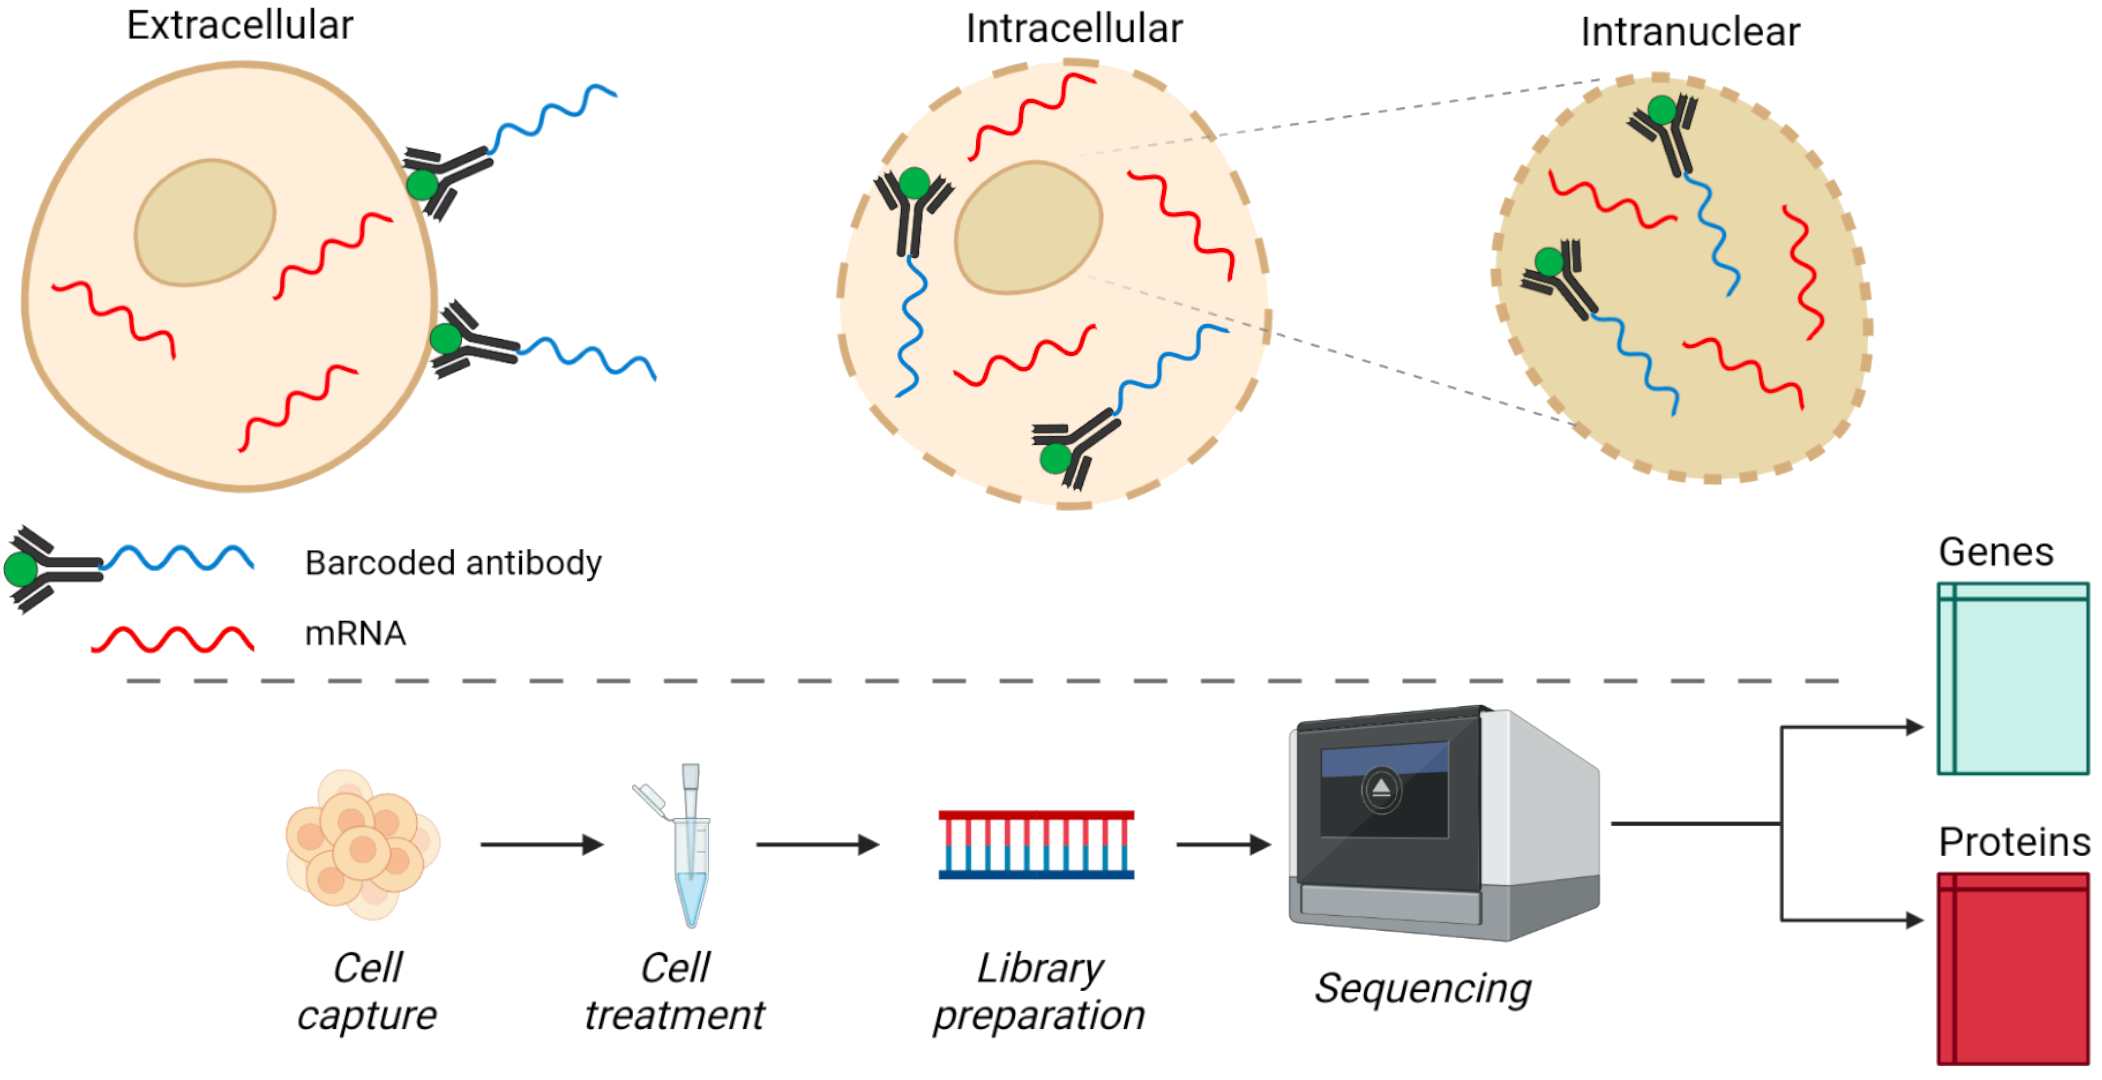
\includegraphics[width=0.8\linewidth]{Figures/LitRev_KR_fig1_v2}
\caption{\textbf{Schematic overview of multimodal single-cell sequencing of genes and proteins.} \textit{(top)} Specific experimental techniques target either extracellular, intracellular or intranuclear proteins simultaneous with transcripts. Antibodies targeting particular proteins are conjugated to DNA or RNA barcodes that are sequenced downstream to quantify protein levels. Intracellular and intranuclear measurements require membrane  permeabilisation before antibodies can enter these compartments, which is visualised here as opened membrane structures. \textit{(bottom)} Abstract wet lab workflow to process single-cells into sequencing readouts of genes and proteins. Cell capture can be droplet- or plate-based, cell treatments may include additional steps to accommodate antibody-binding, library preparation can include cDNA synthesis from RNA as well as cell barcode processing, and sequencing of cell libraries will result in multimodal gene and protein readouts linked to individual cells by shared cell barcodes.}
\label{fig:Figure 1}
\end{figure*}

A visual overview of the multimodal single-cell sequencing techniques for genes and proteins is given in \textbf{Figure} \ref{fig:Figure 1}, and further details on the technical aspects of these experimental techniques are discussed in the sections below.

\subsection*{Extracellular proteins} Thus far the experimental techniques to simultaneously measure proteins and transcripts were limited due to having insufficient reporter molecules or requiring proximity-based protocols for protein binding. FACS has limited numbers of fluorescent labels and mass cytometry is limited in the number of mass labels available \cite{Stoeckius2017}. Other techniques relied on proximity-based protocols with limited capacity for unbiased measurements of larger protein panels \cite{Darmanis2016,Genshaft2016,Albayrak2016}. CITE-seq \cite{Stoeckius2017} and REAP-seq \cite{Peterson2017} implemented innovative antibody-barcoding strategies to expand the size of protein panels. These strategies consist of conjugating antibodies to DNA-barcodes that are captured by primers and subsequently sequenced. \newline \textit{CITE-seq} devised oligonucleotides that included an antibody-barcode and a PCR-handle for amplification. Antibodies are conjugated to two streptavidin tetramers and non-covalently bind the 5’ end of biotinylated oligonucleotides. Single cells are encapsulated in droplets with the Drop-seq protocol \cite{Macosko2015}, after which cell lysis occurs and both mRNAs and antibody-oligonucleotides are then captured on beads, where the bead poly[T]-tail anneals to 3’ poly[A]-tails of mRNAs and antibody-oligonucleotides. These beads contain a PCR-handle together with a cell barcode and Unique Molecular Identifier (\textit{UMI}) to uniquely mark cells and amplification products. Droplet emulsions are broken to reverse transcribe cell contents simultaneously. Importantly, unbound antibodies are washed away before processing. After PCR amplification the mRNA and protein products are size-separated into independent libraries that are sequenced for readouts. \newline \textit{REAP-seq} uses similar oligonucleotides with an antibody-barcode and PCR-handle, however it employs a covalent bond to conjugate antibodies to 5’ ends of aminated oligonucleotides. Here too, unbound antibodies washed away before further processing. The 10x Genomics platform \cite{Villani2017} is used to lyse cells upon encapsulation and then anneals the 3’ poly[A]-tails of mRNAs and antibody-oligonucleotides to poly[T]-tails of conceptually similar beads (with a PCR-handle, cell barcode and UMI), before reverse transcription takes place. Afterwards, the droplet emulsions are broken and the mRNA and protein PCR products can be separated into independent libraries that are sequenced for readouts. \newline Both CITE-seq and REAP-seq are \textit{multiplexed} approaches, meaning that all cell samples are barcode-labelled, mixed together and simultaneously processed in droplet emulsions. Multiplexing increases sample throughput, increases numbers of cells and replicates, and detects multiplet artifacts (multiple cells found in one droplet) to remove. The readout of multiplexed measurements can be computationally \textit{demultiplexed} to identify cells by their sample of origin. The research group that developed CITE-seq also published the \textit{cell hashing} technique \cite{Stoeckius2018}. Cell hashing includes hashtag oligonucleotides (\textit{HTOs}), which are DNA-barcodes for antibodies against proteins that are ubiquitously expressed on cell surfaces, that enables labelling and pooling cells from distinct samples. Demultiplexing is also applied and there are advantages for cell hashing when it is applied in perturbation experiments, where samples are genetically identical \cite{Stoeckius2018}. Other advantages relate to multiplet detection and distinguishing between low-quality cells or empty droplets with ambient RNA. Furthermore, cell hashing can be used to \textit{super-load} cells at higher concentrations to reduce experimental costs. Proof-of-principle experiments in the publications of CITE-seq and REAP-seq used relatively small panels of 13 and 82 antibodies respectively. However, barcodes sufficiently scale to larger antibody panels given the possible number of sequence combinations \cite{Stoeckius2017,Peterson2017}. \newline CITE-seq and REAP-seq characterised human immune cells, for which extensive profiling of single modalities had already been achieved in the past. CITE-seq profiled cord blood mononuclear cells and recovered distinct cell types based on unsupervised clustering of transcriptome data and expression of marker genes. Protein markers for T-cells, B-cells, natural killer cells, monocytes and dendrites were also covered in the specific cell types, along with a rare precursor cell type. Moreover, enhanced characterisation was possible for natural killer cells where the levels of surface proteins CD56 and CD16 revealed subpopulations that would not have been detected from the transcriptome alone. REAP-seq also characterised peripheral blood mononuclear cells (PBMCs) with unsupervised transcriptome clustering, and identified monocytes, B-cells, T-cells and natural killer cell types. Some protein markers could identify immune cell types more sensitively than genes could, although the transcriptome was not neglectable either. On the contrary, certain isoforms could only be detected by protein measurements because their transcripts were not measured. Investigation of pharmacological perturbations with REAP-seq also revealed the utility of surface protein markers to discriminate between treatments. In this experiment, naive CD8+ T-cells from three blood donors were treated with agonist monoclonal antibodies to CD27. While the treatment condition of cells could be identified using protein measurements in all three donors, this was not possible using transcriptome data alone. Additionally, this revealed differential expressed genes and proteins that pointed to biologically relevant mechanisms. In summary, CITE-seq and REAP-seq improved cellular characterisation beyond transcriptomics and results could be experimentally confirmed with gold-standard flow cytometry.

\subsection*{Intracellular proteins} While both CITE-seq and REAP-seq expanded single-cell RNA-sequencing to include protein measurements, and enabled novel investigations into cell types and perturbation responses, the techniques are limited to extracellular proteins. Intracellular proteins involved in the signaling networks that are at the heart of cell functioning were left unprofiled by these techniques. Permeabilisation of cells is an important step to allow antibodies targeting intracellular proteins to cross the cell membrane and additional cell fixation is needed to prevent the loss of cellular mRNAs. These steps have to be incorporated into protocols to simultaneously measure intracellular proteins and transcripts. \newline Key advances were made with \textit{RAID-seq} \cite{Gerlach2019}, in which first cross-linking, fixation and permeabilisation are applied to cells and then antibodies are conjugated to RNA-barcodes. Next, cells are sorted into plates with CELseq2 and SORT-seq protocols \cite{Muraro2016,Hashimshony2016}, in which lysis takes place and reverse-crosslinking causes the release of both mRNAs and antibody-conjugated RNA-barcodes. Reverse transcription follows, together with the preparation and sequencing of merged mRNA and antibody-barcode libraries. \newline The authors of RAID-seq later released \textit{QuRIE-seq}, which offers a high-throughput droplet-based approach for simultaneous transcriptome and intracellular (phospho-)protein measurements \cite{Rivello2020}. QuRIE-seq uses a similar approach of applying cross-linking, permeabilisation and fixation to cells, however it employs DNA-barcodes to tag antibodies. Cells are barcoded and encapsulated into droplets with the inDrop protocol \cite{Klein2015}, followed by reverse-crosslinking and the preparation and sequencing of separate libraries for transcripts and proteins. \newline Proof-of-principle experiments for intracellular techniques focused on signaling networks and their responses to external stimuli. RAID-seq investigated epidermal growth factor (EGF) signaling inhibition in keratinocytes, epidermal skin cells that remain in a stem-cell state due to EGF and integrin contact signaling \cite{Gerlach2019}. Keratinocyte differentiation that migrates cells upwards in the skin requires EGF and integrin signaling inhibition, and RAID-seq captured anticipated differentiation and response heterogeneity in cells that retained hallmarks of integrin signaling. The inclusion of intracellular phosphoprotein levels enabled these findings, particularly analysis of levels between and within treated or untreated cells and consecutive differential expression analysis of transcripts, which underlines the added value of multimodal single-cell data. Furthermore, QuRIE-seq quantified the effects of pharmacological treatment on Burkitt lymphoma cells (cancer of B-lymphocytes) using anti-immunoglobulin antibodies (aIg) that stimulate signaling of the B-cell antigen receptor (BCR) pathway which is characteristic for these cells \cite{Rivello2020}. Combined protein and transcript measurements at multiple time points identified distinct cellular response phases to aIg: response in the initial minutes that is characterised by changing (phospho-)protein levels and response in the range of hours that is marked by gene regulation and processes related to proliferation. Moreover, QuRIE-seq investigated Burkitt lymphoma cells after aIg stimulation together with a BCR signaling inhibitory drug at multiple timescales. Modelling the responses to this treatment revealed the affected signaling components and suggestions of a feedback loop taking place. These modelling approaches are described in more detail in the \textbf{Computational methods} section. \newline RAID-seq initiated the simultaneous capture of intracellular proteins with a panel of 6 RNA-barcoded antibodies and QuRIE-seq expanded this to DNA-barcoded 80 antibodies for intra- and extracellular (phospho-)proteins. Such panels can encompass the components of complex signaling pathways including their phosphorylated forms. Multimodal intracellular measurements enable high-resolution (temporal) characterisation of responses in signaling networks that can be applied to numerous cellular contexts and perturbations. 

\subsection*{Intranuclear proteins} Because the nucleus is a crucial site for gene regulation, expanding techniques to also capture intranuclear proteins can help to further understand cell signaling and gene regulation. In particular, the roles of transcription factors (TFs) and their effects in response to environmental stimuli is relevant. Single-nucleus RNA-sequencing (\textit{snRNA-seq}) protocols address limitations of scRNA-seq, including the need for fresh tissue and loss of cells or transcripts conferred by dissociation steps, yet profiling nuclei is in itself limited by lower mRNA levels and challenges in targeting certain cell types \cite{Slyper2020}. As such, snRNA-seq can be applied to frozen and fragile tissues, and is the evident choice to simultaneously capture protein levels that would aid in characterising gene regulation and cell states. \newline The first technique to simultaneously measure intranuclear proteins and transcripts is \textit{inCITE-seq} \cite{Chung2021}. Nuclei are first fixed and permeabilised for antibody diffusion across the nuclear membrane, and then blocked to reduce non-specific antibody binding. This is followed by droplet encapsulation, nuclei-hashing with an adapted multiplexing approach \cite{Gaublomme2019} and ultimately snRNA-seq of DNA-barcoded antibody and transcript libraries. InCITE-seq assessed several mechanisms: the detection of extracellular induction of TF nuclear translocation, characterisation of mouse brain cells upon drug treatment and modelling effects of TFs on gene expression. First, quantification of antibody-derived p65 levels in response to stimulating cells with cytokine TNF$\alpha$ validated the capability to measure nuclear proteins with inCITE-seq. Second, the mouse hippocampus was characterised after treatment with kainic acid, which induces seizures and activates pathways related to neuronal inflammation and death and oxidative stress. Hippocampal cell types were recapitulated in distinct clusters based on marker gene expression, and compared to a control sample, the authors could identify upregulation of specific pathway components from intranuclear protein levels. Third, inCITE-seq modelled the relative impact of TFs on gene expression and identified putative TF-regulated genes. Modelling co-expression of TF-associated genes in specific cell types also highlighted certain gene modules either upregulated or downregulated by a TF. Altogether, the experimental innovations of inCITE-seq and modelling of its data expand the characterisation of gene regulatory networks. This technique does have limitations as it requires high-quality antibodies due to non-specific binding within the nucleus. Additionally, the study used a limited panel of 4 antibodies which could be expanded to include more (phosphorylated) proteins in future studies \cite{Chung2021}. \newline Following several months after inCITE-seq, \textit{NEAT-seq} extends simultaneous intranuclear protein and transcriptome measurements together with chromatin accessibility \cite{Chen2021}. NEAT-seq employs a creative solution to minimise non-specific antibody binding and incubates the DNA-barcoded antibodies with \textit{E. coli} single-stranded DNA binding protein (\textit{EcoSSB}) to reduce the high negative charge of the conjugate that could drive non-specific binding. Advantageous properties of EcoSSB for intranuclear antibody staining include it having specific single-stranded DNA affinity, slow dissociation and non-interference with PCR amplification. In the NEAT-seq protocol, cells are first fixed and nuclei are isolated and permeabilised, then blocked and stained with EcoSSB-incubated antibody-oligos and followed by PCR amplification of mRNA and protein products before the ultimate capture of all three modalities with the 10x Genomics Multiome kit. NEAT-seq profiled a population of human CD4 memory T-cells with an antibody panel of five key TFs to investigate regulatory activities in specific cell types. Three mechanisms of TF action were highlighted: TFs regulated by transcription levels, TFs that are unable to bind chromatin without help of other TFs, and TFs with post-transcriptional regulation. In particular, this last mechanism was only apparent due to the availability of protein measurements, because protein levels conflicted with transcription levels and suggested other (post-transcriptional) processes at work. Furthermore, genes and accessible chromatin stretches that corresponded to high TF levels identified regulatory elements and target genes for each TF. This approach revealed an interesting example, where the risk allele of a pulmonary disease-associated SNP increased chromatin accessibility for the GATA3 binding site in cells with high GATA3 levels. \newline NEAT-seq offers another interesting application of multimodal single-cell sequencing to investigate complex biological interplay, and further expansion of nuclear antibody panels and combining other modalities would expand the toolkit for researchers. More details of the modelling strategies for inCITE-seq and NEAT-seq can be found in the \textbf{Computational methods} section.

\begin{table*}[h]
\centering
\begin{tabular}{l|l|l|l|l|l l}
\textbf{Technique} & \textbf{Published} & \textbf{Proteins} & \textbf{Barcode} & \textbf{Protocol} & \textbf{\# Antibodies}  \\
\hline
CITE-seq \cite{Stoeckius2017} & 2017 & Extracellular & DNA & Drop-seq \cite{Macosko2015} & 13 \\
REAP-seq \cite{Peterson2017} & 2017 & Extracellular & DNA & 10x Genomics Chromium Controller \cite{Villani2017} & 82 \\
RAID-seq \cite{Gerlach2019} & 2019 & Intracellular & RNA & CELseq2 / SORT-seq \cite{Muraro2016,Hashimshony2016} & 6 \\
ECCITE-seq \cite{Mimitou2019} & 2019 & Extracellular & RNA$^*$ & 10x Genomics Chromium & 49 \\
QuRIE-seq \cite{Rivello2020} & 2020 & Intracellular & DNA & inDrop \cite{Klein2015} & 80 \\
inCITE-seq \cite{Chung2021} & 2021 & Intranuclear & DNA & 10x Genomics Chromium V3 & 4 \\
Perturb-CITE-seq \cite{Frangieh2021} & 2021 & Extracellular & RNA$^*$ & 10x Genomics Chromium V3 & 20 \\
NEAT-seq \cite{Chen2021} & 2021 & Intranuclear & DNA & 10x Genomics Multiome Kit & 5 \\
\end{tabular}
\caption{\textbf{Overview of technical aspects for multimodal single-cell sequencing.} A chronological overview is given, showing that initial techniques targeted extracellular proteins, yet innovations since then have enabled intracellular and intranuclear proteins to be quantified simultaneous with transcripts. DNA barcodes are predominantly used as antibody-conjugate for downstream sequencing. Most techniques utilised droplet-based methods to capture cells, only RAID-seq made use of plate-based methods. \newline $^*$ Multimodal perturbation screens that also capture sgRNAs involved in CRISPR-based gene knockdowns.}
\label{table:Table 1}    
\end{table*}

\subsection*{Perturbation screens} Pertubation experiments can help to understand how specific genes contribute to dysregulated cell functioning, e.g. observing the consequences of targeted gene deactivation can identify affected pathways and could inform treatments. CRISPR interference (\textit{CRISPRi}) is one such approach which exploits the CRISPR system to activate or silence genes by using single-guide RNA (\textit{sgRNAs}) to target genes together with catalytically inactive Cas9 protein (\textit{dCas9}) to block RNA-polymerase functioning in coding regions \cite{Gilbert2013}. With additional modifications, CRISPRi has enabled efficient and targeted gene repression or activation. Furthermore, Perturb-seq \cite{Adamson2016,Dixit2016} enables characterisation of the perturbation consequences at the transcriptome-level. Perturb-seq combines perturbations with scRNA-seq to sequence sgRNAs with RNA-barcodes alongside the transcriptome. \newline Enhanced characterisation of phenotypes was initially implemented by \textit{ECCITE-seq} \cite{Mimitou2019}. CITE-seq is its predecessor and therefore several experimental innovations have been leveraged for ECCITE-seq. First, while most techniques capture 3' ends, ECCITE-seq employs an innovation of CITE-seq to capture 5' ends and thereby addresses particular limitations for 3’ end capture of sgRNAs \cite{Mimitou2019}. Second, custom reverse-transcription primers are incorporated to distinguish mRNA, protein tags and cell hashtags. In total, ECCITE-seq captures six modalities: transcripts, (surface) proteins, sgRNA, sample identity from cell hashing \cite{Stoeckius2018}, and clonotypes of T-cell receptor (TCR) $\alpha$/$\beta$ and of TCR $\gamma$/$\delta$. ECCITE-seq proved capable of resolving cellular origins from multimodal data in a mixture of human PBMCs, human T-cell lymphoma cell lines and a sgRNA-targeted mouse cell line. In this cell mixture, cell hashtags differentiated samples, antibodies differentiated between species, TCR clonotypes were resolved only in the human cells, and sgRNAs were only recovered in mouse cells. In another experiment, the effect of inhibited gene expression for sgRNA-targets could be measured and the collapse of relevant protein levels was even more pronounced. TCR clonotype detection lends ECCITE-seq to study the heterogeneous repertoire of TCRs and their functional impacts \cite{Nathan2019,Zhang2021}. \newline More recently \textit{Perturb-CITE-seq} \cite{Frangieh2021} was published, which extends CRISPR perturbations to large screens and comprehensive computational analysis of the multimodal data. This technique is also based on CITE-seq and combines droplet-based 3’ capture with sgRNA-targeting to knockout genes. While the captured modalities are not as extensive as ECCITE-seq, Perturb-CITE-seq provides an approach for large perturbation screens with an extended computational framework to investigate the impact of perturbations. As a proof-of-concept, Perturb-CITE-seq investigated resistance to immune checkpoint inhibitors in melanoma immunotherapy with a dataset of more than 200,000 cells, 20 surface proteins and sgRNAs targeting 248 genes putative to confer resistance. The experimental design included control cells, IFN-$\gamma$ treated cells and co-cultured cells with tumor infiltrating lymphocytes (TILs, patient-derived cells altered to target the tumor itself). As such, the impact of perturbations on IFN-$\gamma$-JAK/STAT signaling involved in immune response and TILs could be assessed. Not only could particular alterations of mRNA or protein levels be detected and related to known pathways, the computational integration of multimodal data offers a rich source of information regarding the resistance mechanisms (more details in the \textbf{Computational methods} section). Modelling the effects of individual perturbations on mRNA and protein levels recapitulated the key modules of cancer immune evasion and also discovered new modules beyond IFN-$\gamma$-JAK/STAT and TIL mechanisms that could be involved. Furthermore, their approach identified a novel gene target with roles in immune evasion. These results highlight the promise of Perturb-CITE-seq to elucidate the complex mechanisms of numerous other diseases. Expansion of multimodal single-cell perturbation screens to other relevant cellular markers (e.g. chromatin accessibility) and diseases could turn it into an application of single-cell multimodal techniques with substantial impact for patient treatment.

\subsection*{Perspective} Innovations in multimodal single-cell technologies have rapidly followed in recent years, as both the captured modalities and accessible cellular components have been expanded. An overview of several technical aspects per technique is given in \textbf{Table} \ref{table:Table 1}. Data for scRNA-seq is characterised by frequent dropouts events, where the majority of genes in cells have zero observed transcripts and are only expressed in some cells. As a consequence of this, scRNA-seq data is highly sparse and quality control steps to address this are commonplace in scRNA-seq analysis \cite{AlJanahi2018}. Discussions on the nature of scRNA-seq dropouts involve how sparsity should be addressed, and how to distinguish between true signals, e.g. low mRNA levels in cells and the stochastic nature of gene expression, and measurement errors \cite{Qiu2020,Sarkar2021}. However, a different pattern emerges from protein-level data obtained with the techniques discussed here: proteins tend to display more stable levels and have lower dropout rates \cite{Stoeckius2017,Peterson2017,Gerlach2019,Mimitou2019}. Moreover, low correlation between the levels of encoding genes and produced proteins has been found \cite{Stoeckius2017,Peterson2017}. This could however reflect inflation from multiple DNA-barcodes conjugating to an antibody. For instance, REAP-seq reported an average of three barcodes per antibody \cite{Peterson2017}. Protein dynamics have also been put forward as a potential explanation: proteins have longer half-lives and higher absolute abundance, while mRNA is more constantly being degraded \cite{Schwanhusser2011}. \newline Antibody panel sizes have remained relatively limited compared to the coverage of genes, however in most publications discussed here prior knowledge informed the antibody selection, e.g. for immune cell types \cite{Stoeckius2017,Peterson2017}. Additionally, numerous experiments reviewed here highlighted that including measurements for limited numbers of antibodies could enhance cellular characterisation nonetheless. The experimental techniques reviewed here cover panels with only a few antibodies, such as RAID-seq \cite{Gerlach2019}, towards more than eighty antibodies with REAP-seq \cite{Peterson2017} and QuRIE-seq \cite{Rivello2020}, and panel sizes are summarised in \textbf{Table} \ref{table:Table 1}. CITE-seq datasets are scaling to ever greater sizes, with one dataset covering over 200,000 human PBMCs and 228 measured antibodies \cite{Hao2021}. Furthermore, the authors of QuRIE-seq suggested that panels would be able to expand to over five hundred antibodies \cite{Rivello2020}. In general, antibody measurements can be limited by biases or antibodies or by non-specific binding. Nuclear antibody panels remain limited due to particular challenges with non-specific antibody binding \cite{Chung2021,Chen2021}, while innovations such as EcoSSB in the NEAT-seq protocol could address technical challenges. 

\section*{Computational methods accommodate novel single-cell research}

\subsection*{Integration}
Multimodal single-cell sequencing is applied for research in diverse biological contexts and several proof-of-principle experiments have emphasised the need for tailored computational analyses. Initial multimodal data were subjected to \textit{sequential analysis}, i.e. distinct modes of data were analysed separately and afterwards brought together for interpretation. An example is CITE-seq, where cell types were determined by transcriptome-based clustering and afterwards protein levels were projected onto cells for enhanced characterisation \cite{Stoeckius2017}. While this approach is attainable with human immune cells for which there is extensive prior knowledge on surface protein markers, translation to other biological settings that are insufficiently characterised is not straightforward. Instead, the informational contribution of additional modalities should be delineated during computational analysis and employed for more comprehensive cellular characterisation. Additionally, sequential analysis will become limiting as antibody panels expand and the demand for automatised computational workflows becomes larger. Instead, \textit{integrative analyses} that can account for varying information content of modalities are of interest to deal with expanding multimodal single-cell datasets. Furthermore, distinct coverage per modality, differences in data quality such as technical bias and noise, and complex experimental setups including time-series, conditions and batches should be taken into account. Both T-distributed Stochastic Neighbor Embedding (\textit{t-SNE}) \cite{vanderMaaten2008} and Uniform Manifold Approximation and Project (\textit{UMAP}) \cite{McInnes2018} are frequently used for dimensional reduction and visualisation of (multimodal) single-cell datasets, yet both have objectives to find low-dimensional representations of cells that capture single modalities and do not properly account for relative contributions of multiple modalities. \newline The computational workflows MOFA+, totalVI and WNN \cite{Argelaguet2020,Gayoso2021,Hao2021} are recent developments for multimodal single-cell data that all learn some latent space representation which captures relevant variation in the data while accounting for the relative contributions per modality. From this latent space, cells can be characterised in downstream analyses that attempt to capture commonalities between similar types of cells, including clustering, differential expression analysis, visualisation and more. Methods rely on different statistical and computational approaches: for instance MOFA+ employs factor analysis to infer latent factors with modality weight matrices to explain variation \cite{Argelaguet2020}, totalVI uses deep learning \textit{variational autoencoders} (\textit{VAEs}) to learn a joint probabilistic representation of RNA and proteins \cite{Gayoso2021}, and WNN learns cell-specific modality weights that reflect relative information content through an unsupervised analysis of neighboring cells \cite{Hao2021}. MOFA+ and totalVI can be classified as \textit{early integration} methods because features from multiple modalities are integrated into one latent representation, while WNN belongs to \textit{late integration} as RNA and protein data are independently analysed before integration \cite{Adossa2021}. Each method is discussed in more detail below. \newline \textit{MOFA+} (Multi-Omics Factor Analysis v2) \cite{Argelaguet2020} is the continuation of the MOFA statistical network \cite{Argelaguet2018} for integrative multimodal analysis, and it addresses certain assumptions and technical challenges related to scalability and inability to deal with complex experimental groups of MOFA. MOFA+ can handle large datasets and multiple modalities from multiple conditions. The inputs are separate datasets where features and cells have aggregated non-overlapping sets of modalities (e.g. RNA, protein and more) and groups (e.g. conditions or batches), respectively. Briefly, MOFA+ trains a model by using a Bayesian prior structure to capture variation shared across multiple modalities, and induces sparse solutions for factors and weights that facilitate model interpretation. Throughout model training, a small number of latent factors for samples are inferred together with feature weight matrices per modality. For instance, factors could explain variation between cell types or between developmental stages and weights are a measure of feature importance, such as a specific gene or protein. The model output includes variance decomposition and feature weights for extensive interpretation, as well as numerous downstream analyses: clustering, feature selection, differentiation trajectory inference and gene set enrichment analysis. Additionally, model factors can be the input for t-SNE or UMAP visualisation. While the original MOFA+ publication already offered various proof-of-principle experiments in cell type commitment or methylation signatures reflecting cellular diversity, a notable multimodal application of MOFA+ is for pharmacological perturbation of Burkitt lymphoma cells across time points with QuRIE-seq \cite{Rivello2020}. Here, cells were treated with anti-immunoglobulin antibody (aIg) and at respectively 0, 2, 4, 6, 60 and 180 minutes after treatment, transcriptome and intracellular (phospho-)protein measurements were taken using the QuRIE-seq protocol. MOFA+ factor analysis enabled the identification of distinct cellular response phases to aIg: factor 1 captured the short-term response (0-2 minutes) with changing (phospho-)protein levels, while factor 3 captured long-term response (1-2 hours) that was typified by gene regulation and processes related to proliferation \cite{Rivello2020}. These findings reflect the key advantages of MOFA+, namely handling complex experimental groups like time-series and facilitating biological interpretation with downstream analyses such as factor and feature inspection. MOFA+ has certain limitations, of which the most relevant here are that only moderate non-linear relationships can be addressed and that the prior distribution assumes feature independence, while genes and proteins can interact through regulatory mechanisms \cite{Argelaguet2020}. Regarding the non-linear relationships, the authors suggested that VAE frameworks could be useful. Briefly, VAEs train models that first “encode” input data into a probability distribution in latent space, and then “decode” points sampled from this distribution to output parameters of the input probability distribution, all in an effort to accurately reconstruct the input. In practice, VAEs can learn a latent representation of single-cell data by modelling the joint probabilities of modalities, and it is this approach that is employed by totalVI. \newline \textit{TotalVI} (Total Variational Inference) \cite{Gayoso2021} expands on the scVI framework for RNA data \cite{Lopez2018} and accounts for paired protein and transcriptome measurements from CITE-seq. Important considerations are different data distributions for RNA and proteins, along with other modality-specific biases and noise. Protein data can be separated into foreground and background signal, the latter is an experimental consequence of ambient or non-specific binding antibodies, and has previously been addressed in CITE-seq with spike-in control cells to establish a baseline for foreground signal \cite{Stoeckius2017}. TotalVI models paired transcript and protein readouts from CITE-seq into a joint probabilistic representation encompassing both biological variation and technical variation (e.g. noise, bias, batch effects), using a deep generative model. Inputs to the model are RNA and protein counts matrices, together with a matrix of batch effects. Two particular components can be derived with totalVI: the first component encodes inputs into a latent cell representation that is informed by distributions of RNA and proteins, the second component decodes from the latent cell representation to estimate likelihoods for genes and proteins for the input. Protein and RNA information are brought together in the latent cell representation, which can be used for cell clustering or visualisation with UMAP. Genes and proteins can be investigated in more detail with the second component, e.g. differential expression analyses or discerning between protein foreground and background. The authors used a CITE-seq dataset of > 30,000 murine spleen and lymph node cells containing heterogeneous immune cell types to evaluate totalVI’s performance. To identify protein background signal, the second component employs a protein mixture model for both foreground and background signal, and totalVI takes cell-specific factors from the latent cell representation into account. Cell type identification that relied on only the foreground signal of several marker proteins performed well and outperformed a simplified baseline in certain cell types. Additionally, the authors argued that removing the protein background signal revealed the presence of technical noise in CITE-seq and REAP-seq where low gene-protein correlations were reported \cite{Stoeckius2017,Peterson2017}, since background-corrected gene-protein correlations from totalVI increased in magnitude compared to uncorrected correlations. Furthermore, totalVI offers protein integration between datasets where missing proteins can be imputed from the observations in another dataset, an approach that relies on the latent representation of the latter dataset. Overall, totalVI offers a comprehensive computational framework for CITE-seq data that includes diverse downstream analyses. \newline \textit{WNN} (Weighted-Nearest Neighbor) analysis is the most recent integrative computational method and it is implemented in the popular Seurat R package for single-cell analysis \cite{Hao2021}. WNN handles multimodal data such as CITE-seq and was designed to deal with varying data quality between modalities, to connect to downstream analyses and to improve cell characterisation beyond sequential analysis. Through an unsupervised approach, WNN calculates modality weights that reflect the information content of modalities per cell. The inputs to WNN are RNA and protein count matrices, which are preprocessed following Seurat standards and are then subjected to dimension reduction with PCA. Per cell, the 20 nearest neighbors are determined for each modality and used to predict the cell's RNA or protein content. RNA and protein weights are calculated to reflect the prediction accuracy and will sum to 1, thus summarising the relative modality contribution per cell. As the output, a graph representation of cells named a \textit{WNN graph} is calculated to integrate modalities. This WNN graph is suitable for various downstream analyses, including t-SNE and UMAP visualisation and clustering. The method was evaluated using a CITE-seq dataset of > 30,000 human bone marrow cells with 25 antibodies and WNN integration demonstrated improved cell type characterisation, particularly in challenging T-cell groups that remained unresolved after transcriptome-based clustering. Additionally, the results highlighted certain cell populations with predominantly high RNA weights or high protein weights, which can inform which modality is most informative to identify particular cell types. Furthermore, WNN provided a benchmark against MOFA+ and totalVI and exhibited that WNN had equivalent or superior performance in inferring molecular states of cells from nearest neighbors. Beyond this CITE-seq experiment, other proof-of-principle experiments with simultaneous transcriptome and chromatin accessibility measurements and ECCITE-seq substantiated the method's capability of extensive characterisation of (previously undetected) cell types. Other positive aspects to this method are its transfer learning procedure to map single-cell datasets to multimodal reference datasets that can advance cell atlas consortia, and that datasets of three or more modalities can also be analysed. \newline The innovations in integrative computational methods offer researchers a variety of approaches to investigate multimodal single-cell datasets. The authors of WNN benchmarked their method against MOFA+ and totalVI, and translated the respective learned latent spaces of these methods to nearest-neighbor graphs akin to the WNN graph \cite{Hao2021}. By doing so the authors posited an interesting approach to further benchmark the methods with more datasets. The particular strengths and weaknesses of these methods regarding accurately characterising particular protein markers should be further explored and could motivate the selection of which computational workflow to use for a particular dataset. There are differences between the downstream analyses included per method, all implement t-SNE or UMAP to visualise or cluster cells and all offer some form interpretation of the latent space: MOFA+ with variance decomposition and feature weight inspection, totalVI with archetypal analysis of gene and protein analysis, and WNN with RNA and protein modalities. Denoising data and accounting for complex experimental groups such as batches are included for MOFA+ and totalVI. Differential expression analysis and the integration of datasets can be handled by totalVI and WNN, while both MOFA+ and WNN can infer cellular trajectories. TotalVI has the unique functionality of decoupling the protein foreground and background, and gene set enrichment analysis is a distinct feature of MOFA+. Furthermore, other integrative methods have been developed and in some instances were evaluated for other multimodal combinations, that could be leveraged for simultaneous transcriptome and protein measurements, e.g. scMVAE, bindSC, Schema, MATCHER, bremSC and CiteFuse \cite{Zuo2020,Dou2020,Singh2021,Welch2017,Wang2020,Kim2020}.

\subsection*{Modelling}
Several modelling strategies have been devised for single-cell multimodal data to investigate cellular dynamics, and key developments in the modelling of transcription and translation dynamics as well as perturbation responses are discussed here. With the inclusion of protein measurements alongside those of transcripts, multimodal datasets extensively cover components of the central dogma. Furthermore, protein measurements of transcription factors (\textit{TFs}), key regulators of gene expression, have been included in recent innovative experimental techniques \cite{Chung2021,Chen2021}. \newline Multimodal single-cell datasets can untangle which genes and proteins drive the differentiation trajectories of precursor cells to differentiated cells. Numerous trajectory inference methods have been developed since the advent of scRNA-seq \cite{Saelens2019}, and the previously described methods MOFA+ and WNN offer trajectory inference as one of their downstream analyses. More recently, the concept of \textit{RNA velocity} was introduced, which presents extensive kinetic modelling of transcriptional dynamics and enables prediction of future cellular states \cite{LaManno2018}. The ratios of spliced and unspliced mRNAs from genes are used to calculate RNA velocity as the time derivative of gene expression. In a model with the following genic processes: transcription ($\alpha$), splicing ($\beta$) and degradation ($\gamma$), and the following products: unspliced mRNA ($u$) and spliced mRNA ($s$), RNA velocity is defined as $\frac{ds(t)}{dt} = \beta u(t)-\gamma s(t)$ where a common gene splicing rate $\beta$ is assumed. Steady-state transcriptional equilibria are assumed to be attained after phases of gene activation and repression of sufficient duration. Positive RNA velocity states ($u > \gamma s$) represent gene activation, reflecting the recently increased fraction of unspliced transcripts, and vice versa negative RNA velocity states ($u < \gamma s$) represent gene repression. In a population of differentiating cells, RNA velocity can be used to extrapolate the future state of individual cells and cell types over the course of hours, and be projected in low-dimensional embeddings such as PCA or t-SNE. Cells can simultaneously have RNA velocities over several components, such as proliferation or differentiation. Proof-of-principle applications of RNA velocity included predicting the circadian rhythm progression or tracking murine hippocampal cells maturing from neuroblasts to distinct branches of neuronal and glial cell types. Limitations stated by the authors included the assumption of steady-state models with one common splicing rate for genes, and they cautioned that substantial velocity in one embedding is not always seen in the other, so that PCA and t-SNE visualisation should be interpreted with care. \newline A dynamical model was presented by another research group with the \textit{scVelo method} to generalise RNA velocity and to address limitations of the steady-state model in cases where heterogeneous cell subpopulations have different kinetics \cite{Bergen2020}. The dynamical model relies on an expectation-maximisation (\textit{EM}) framework to iteratively infer parameters under maximum likelihood: first the cell-specific discrete transcriptional states and latent time, and second the gene-specific transcription, splicing and degradation rates. Ultimately, scVelo accounts for gene-specific splicing rates in RNA velocity as $\frac{ds(t)}{dt} = \beta u(t)-\gamma s(t)$. The advantages are that the resulting gene trajectories have interpretable rates and transcription states that describe RNA levels over (latent) time, and the EM model yields gene likelihoods that enable identification of driver genes underlying dynamic processes such as differentiation. In one application, both scVelo and the steady-state model are applied to a population of developing mouse hippocampal (dentate gyrus) cells. Although both capture major differentiation processes from developing to mature cell types, scVelo resolves terminal cell types and removes velocity accordingly, unlike the steady-state model. Overall, scVelo appears to yield more coherent velocities and similar cells tend to have better correlated velocities. This model does have limitations due to its assumptions of gene-specific splicing and degradation rates being constant, and there being only two transcription rates for gene activation and repression, respectively. In a recent review, several examples of genes with complex kinetic dynamics that defied model assumptions illustrated these limitations \cite{Bergen2021}. Future implementations should account for more complex gene regulation mechanisms and other gene properties, together with incorporating other modalities \cite{Bergen2020, Bergen2021}. Furthermore, the authors suggested applying scVelo to characterise perturbation responses. Hypothetically, cells from before and after pharmacological treatment are investigated and generalised RNA velocity could characterise susceptible and resistant cell types, as well as driver genes. \newline The concept of \textit{protein velocity} benefits from multimodal datasets that enable the original steady-state RNA velocity model and its assumptions to be extended to include protein translation and degradation \cite{Gorin2020}. Conceptually, the model adds the processes of protein translation ($\beta _p$) and degradation ($\gamma _p$), adds protein ($p$) as product, and defines protein velocity as $\frac{dp(t)}{dt} = \beta _p s(t) - \gamma _p p(t)$ where similar to RNA velocity one common translation rate $\beta _p$ is assumed. Information contained in the spliced transcript population allows the model to predict past and future cell states. Additionally, the combination of protein velocity and underlying RNA velocity are used to estimate \textit{protein acceleration} to project onto a low-dimensional embedding. The method was applied to six multimodal datasets of PBMCs from CITE-seq, REAP-seq, ECCITE-seq (healthy control and cutaneous T cell lymphoma patient) and 10x Genomics (1000 cells and 10,000 cells), with some dozens of measured proteins. Strong velocity signals were observed in CITE-seq and 10x Genomics, in contrast to REAP-seq and ECCITE-seq where noisy or sparse acceleration was observed. The authors offered reduced RNA libraries for the latter two techniques as a potential technical confounder. Similar to arguments made by Bergen et al. for generalised RNA velocity \cite{Bergen2020}, assumptions of common splicing and translation rates could be limitations to protein velocity. Generalised forms of t-SNE and UMAP (\textit{j-SNE} and \textit{j-UMAP}) were recently postulated and evaluated for RNA and protein velocity embeddings \cite{Do2021}. Both j-SNE and j-UMAP are adapted to overcome limited representations learned from single modalities and instead learn joint representations of multiple modalities. The authors noted that previous projections of RNA and protein velocities were limited because of their transcriptome-based t-SNE embedding, and the authors repeated analyses with j-SNE and j-UMAP. This corrected ECCITE-seq and REAP-seq acceleration landscapes, which afterwards displayed aligned cell types rather than mixed cell types. Two potential explanations for noisier landscapes with protein velocity were given: larger antibody panels of ECCITE-seq and REAP-seq compared to CITE-seq and 10x Genomics led to further subdivided cell types, and this was reflected by considerable lower agreement between RNA and protein cluster results for ECCITE-seq than for CITE-seq. Thus, disagreement between RNA and protein measurements could affect protein acceleration calculations and joint representations could reduce discrepancies when the embedding is visualised \cite{Do2021}. Nonetheless, protein velocity results with CITE-seq and 10x Genomics datasets appear promising and warrant further development of transcriptional and translational dynamics modelling with multimodal data that aid in cellular characterisation and understanding developmental processes and perturbation responses. \newline Further modelling was conducted with inCITE-seq, in which the intranuclear measurements of transcripts, the TFs p65, c-Fos and PU.1, and neuronal marker NeuN were leveraged to model gene expression as a function of TF levels and to identify co-expressing gene modules for each TF \cite{Chung2021}. Genes associated with p65 levels were modelled with the following variables; $Y_i$ are counts of gene $i$, $p65$ are p65 protein levels, $G2M$ and $S$ are cell cycle scores calculated from known cell cycle genes, and $log(UMI)$ and $log(HTO)$ are counts of UMIs and nuclei hashtags respectively, in a generalised linear model with negative binomial fit: $Y_i \sim p65 + G2M + S + log(UMI) + log(HTO)$. With this linear modelling and Benjamini-Hochberg FDR correction, significant positive associated genes for p65 levels could be identified and contextualised in pathways with known involvement of p65. Similarly, surveyed mouse hippocampus cells were used to find putative TF-regulated genes with a two-step mixed linear model. First, with the following variables: $Y_i$ as Z-score scaled counts for gene $i$, $C _{(cluster)}$ and $C _{(treatment)}$ as categorical variables of cell cluster and treatment, and $log(UMI)$ and $log(HTO)$ identical to before, gene expression was modelled to regress out cell cluster and treatment covariates: $Y_i \sim C _{(cluster)} + C _{(treatment)} + C _{(cluster)}*C _{(treatment)} + log(UMI) + log(HTO)$. Second, resulting gene residuals $rY_i$ were modelled as the combination of all proteins: $rY_i \sim cFos + p65 + NeuN + PU.1$. To aid interpretability, the effect sizes for each protein were estimated from the model coefficients, for instance to detect significant positive associated genes. Finally, calculating the Pearson correlations of gene expression for specific genes with positive or negative TF associations, followed by ordering with hierarchical clustering revealed co-expressed gene modules. Overlaying gene modules with the TF effect sizes for genes in the modules can further aid the interpretation. Altogether, multimodal single-cell datasets enable this type of modelling that provides insights into the relative contributions of TFs to gene expression \cite{Chung2021}. \newline The authors of Perturb-CITE-seq developed a computational framework to analyse multimodal perturbation screens, which models effects on RNA and protein levels and identifies perturbed gene modules that impact gene and protein programs through induction or reduction \cite{Frangieh2021}. First, highly variable and jackstraw PCA-selected genes and all measured proteins were selected for each of three experimental conditions, and second, linear models learned the effects of each perturbed gene on all gene and protein features, which included elastic net regularisation and covariates for cell quality and cell cycle state. Furthermore, their approach calculated Pearson correlations between perturbed genes and between RNA and protein features, followed by transformation into empirical P values of genes and proteins for all perturbed genes. Finally, this enabled clustering of perturbed genes to identify modules and clustering of genes and proteins to identify programs, respectively. Perturb-CITE-seq identified eight modules of gene perturbations that affected one or more of four programs in melanoma, which also presented new modules beyond the previously characterised mechanisms of immune evasion. It would therefore be promising to conduct Perturb-CITE-seq experiments in other contexts to hopefully uncover more disease mechanisms through its computational framework.

\section*{Discussion and conclusion}

Sequencing methods that capture multiple modalities of biological data are crucial to research the complex mechanisms of cells, including characterisation of cell states, dynamics and responses to environmental or pharmacological perturbations. Numerous single-cell sequencing techniques have been developed in past years for multiplexed measurements of transcripts and extracellular proteins; CITE-seq \cite{Stoeckius2017}, REAP-seq \cite{Peterson2017}, RAID-seq \cite{Gerlach2019}, ECCITE-seq \cite{Mimitou2019} and Perturb-CITE-seq \cite{Frangieh2021}, intracellular proteins; RAID-seq \cite{Gerlach2019} and QuRIE-seq \cite{Rivello2020}, and intranuclear proteins: inCITE-seq \cite{Chung2021} and NEAT-seq \cite{Chen2021}. Experiments conducted with these techniques have contributed to unraveling new cell subpopulations, characterising perturbation responses in signaling networks, investigating TF-mediated gene regulation, and more. However, experimental limitations related to antibody binding, cell compartment accessibility and addressing technical variation are present in these techniques and should be the subject of further innovations. Ambient antibodies from empty droplets in particular, together with non-specific antibody binding and technical aspects such as high antibody concentrations have been attributed to noise in CITE-seq data and can be corrected for \cite{Mule2020,Buus2021}. Besides this, totalVI can computationally model modality-specific noise such as protein background and correct for this \cite{Gayoso2021}. Expansion of measurements from the cell surface to the inside of cells and their nuclei presents unique technical challenges that permeabilisation and fixation techniques address \cite{Gerlach2019,Rivello2020,Chung2021,Chen2021}, and creative strategies including that of NEAT-seq to reduce non-specific antibody binding with an \textit{E. coli} protein will be important for future innovations. Furthermore, super-loading of cells with cell hashing \cite{Stoeckius2018} scales high-throughput experiments even further and reduces costs, and facilitates expansions to more modalities with modality-specific hashtags \cite{Mimitou2019}. \newline Integrative computational methods have expanded multimodal data analysis beyond sequential analysis, with early integration methods MOFA+ and totalVI, and WNN for late integration, to learn latent representations of cells. These methods can be limited by their assumptions or the type of detectable relationships. Thus far, these methods have only been benchmarked for performance and runtime in one particular CITE-seq dataset \cite{Hao2021}. While WNN outperformed MOFA+ and totalVI for particular proteins, additional benchmarking is needed to determine the generalisability to other datasets. Furthermore, WNN exhibited lower runtimes to analyse the entire dataset than MOFA+ and totalVI did, which could be a relevant consideration as future datasets increase in their numbers of measured cells. Modelling RNA velocity in steady-state and dynamical models has provided insights into cell state transitions over time, such as cell type differentiation in the developing mouse brain. Current protein velocity warrants further development, model assumptions could be updated akin to the dynamical RNA velocity model, and noise in multimodal data has to be addressed accordingly. As shown with scVelo, even the adapted model can eventually be defied by biological exceptions \cite{Bergen2021}, and future implementations of protein velocity should also accommodate rare, complex mechanisms. Furthermore, the concept of chromatin potential that utilises multimodal RNA and chromatin accessibility data to infer future transcriptomic states from chromatin states expands the modelling landscape \cite{Ma2020}. As the latest innovations of TEA-seq \cite{Swanson2021} and DOGMA-seq \cite{Mimitou2021} consolidate simultaneous transcriptome, protein and chromatin accessibility measurements, future modelling approaches could help to connect the molecular interactions involved in cell function and regulation. \newline This review has focused on simultaneous single-cell sequencing of transcripts and proteins, however there have been concurrent innovations to simultaneously capture chromatin accessibility, DNA methylation or spatial information. In the timespan of merely five years there have been major innovations in single-cell techniques, and it can only be hoped that this trend will continue to help researchers to further decipher the complex mechanisms of cells.

\begin{acknowledgements}
I would like to thank Dr. Evert Bosdriesz for the opportunity to conduct this literature review and for his supervision and feedback. Additionally, I want to thank the department of Bioinformatics at Vrije Universiteit Amsterdam for their support and for providing an adequate and welcoming workplace.
\end{acknowledgements}

\section*{Bibliography}
\bibliography{multimodal-single-cell}

%% You can use these special %TC: tags to ignore certain parts of the text.
%TC:ignore
%the command above ignores this section for word count
\onecolumn
\newpage

%%%%%%%%%%%%%%%%%%%%%%%%%%%%%
% Supplementary Information %
%%%%%%%%%%%%%%%%%%%%%%%%%%%%%
%\captionsetup*{format=largeformat}
%\section{Something about something} \label{note:Note0} 
%\Blindtext

%TC:endignore
%the command above ignores this section for word count

\end{document}